\documentclass[11pt]{article}
\usepackage{amsmath,amssymb,enumitem,algorithm,algpseudocode}
\usepackage{tikz}
\usepackage[UTF8]{ctex}
\usepackage[braket]{qcircuit}
\parindent=22pt
\parskip=3pt
\oddsidemargin 18pt \evensidemargin 0pt
\leftmargin 1.5in
\marginparwidth 1in \marginparsep 0pt \headsep 0pt \topskip 20pt
\textheight 225mm \textwidth 148mm
\renewcommand{\baselinestretch}{1.15}
\begin{document}
\title{{\bf 理论作业三 \quad 量子编译与量子纠错}}
\author{周楠 \quad 3220102535}
\date{\today}
\maketitle

\begin{tabular*}{13cm}{r}
\hline
\end{tabular*}

\vskip 0.3 in

{\bf 1.} 已知双量子比特电路对应矩阵如下:
\begin{align*}
    U = \begin{pmatrix}
    1 & 0 & 0 & 0 \\
    0 & -1 & 0 & 0 \\
    0 & 0 & 0 & 1 \\
    0 & 0 & -1 & 0 \\
    \end{pmatrix}
\end{align*}
\begin{enumerate}[label=\alph*.]
    \item 证明矩阵 $U$ 是一个合法的酉矩阵。
    \[
    UU^\dagger = 
    \begin{pmatrix}
        1 & 0 & 0 & 0 \\
        0 & -1 & 0 & 0 \\
        0 & 0 & 0 & 1 \\
        0 & 0 & -1 & 0 \\
    \end{pmatrix}
    \times
    \begin{pmatrix}
    1 & 0 & 0 & 0 \\
    0 & -1 & 0 & 0 \\
    0 & 0 & 0 & -1 \\
    0 & 0 & 1 & 0 \\
    \end{pmatrix} = 
    \begin{pmatrix}
    1 & 0 & 0 & 0 \\
    0 & 1 & 0 & 0 \\
    0 & 0 & 1 & 0 \\
    0 & 0 & 0 & 1 \\
    \end{pmatrix} = I
    \]
	\item 将酉矩阵 $U$ 分解为尽可能少的基础量子门(CNOT、X、Y、Z)组合,并画出相应的量子电路图。
	\[
    U |00\rangle = \begin{pmatrix}
    1 & 0 & 0 & 0 \\
    0 & -1 & 0 & 0 \\
    0 & 0 & 0 & 1 \\
    0 & 0 & -1 & 0 \\
    \end{pmatrix}
    \times
    \begin{pmatrix}
    1 \\
    0 \\
    0 \\
    0 \\
    \end{pmatrix} = \begin{pmatrix}
    1 \\
    0 \\
    0 \\
    0 \\
    \end{pmatrix} = |00\rangle
    \]
    \[
    U|01\rangle = -|01\rangle\\
    \]
    \[
    U|10\rangle = -|11\rangle\\
    \]
    \[
    U|11\rangle = |10\rangle
    \]
    对应的电路图为:
    \[ \Qcircuit @C=1.0em @R=1.5em {
    \lstick{q_0} &  \qw & \ctrl{1}  & \qw & \qw \\
    \lstick{q_1} &  \qw & \targ  & \gate Z  & \qw 
    } \]
\end{enumerate}

\vskip 0.3 in

{\bf 2.} 给定一包含 5 个物理量子比特的量子处理器,其量子比特间的耦合连接关系如下:
\begin{center}
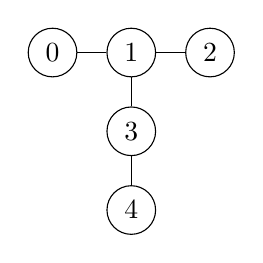
\begin{tikzpicture}
    \node[circle, minimum width=15pt, minimum height =15pt, draw=black] (1) at (-1,0) {$0$};
    \node[circle, minimum width=15pt, minimum height =15pt, draw=black] (2) at (0,0) {$1$};
    \node[circle, minimum width=15pt, minimum height =15pt, draw=black] (3) at (1,0) {$2$};
    \node[circle, minimum width=15pt, minimum height =15pt, draw=black] (4) at (0,-1) {$3$};
    \node[circle, minimum width=15pt, minimum height =15pt, draw=black] (5) at (0,-2) {$4$};
    \draw[-] (1) -- (2);
    \draw[-] (2) -- (3);
    \draw[-] (2) -- (4);
    \draw[-] (4) -- (5);
\end{tikzpicture}
\end{center}

现有一包含 5 个逻辑量子比特的量子电路如下:
\[ \Qcircuit @C=1.0em @R=1.5em {
\lstick{q_0} & \ctrl{1} & \ctrl{2} & \ctrl{3} & \ctrl{4} & \qw & \qw & \qw \\
\lstick{q_1} & \control \qw & \qw & \qw & \qw & \ctrl{2} & \qw & \qw \\
\lstick{q_2} & \qw & \control \qw & \qw & \qw & \qw & \ctrl{1} & \qw \\
\lstick{q_3} & \qw & \qw & \control \qw & \qw & \control \qw & \control \qw & \qw \\
\lstick{q_4} & \qw & \qw & \qw & \control \qw & \qw & \qw & \qw 
} \]

给出将这个逻辑量子电路部署至量子处理器时的量子比特映射关系,以插入最少的 SWAP 门使得每个双量子比特门都能直接在相连的物理量子比特间执行。

量子比特的初始映射关系为:
\[ q_0 \rightarrow 1, q_1 \rightarrow 2, q_2 \rightarrow 3, q_3 \rightarrow 4, q_4 \rightarrow 0 \]
\begin{center}
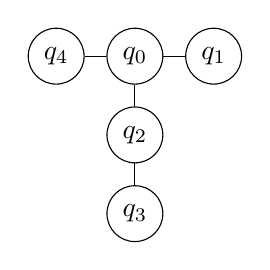
\begin{tikzpicture}
    \node[circle, minimum width=15pt, minimum height =15pt, draw=black] (1) at (-1,0) {$q_4$};
    \node[circle, minimum width=15pt, minimum height =15pt, draw=black] (2) at (0,0) {$q_0$};
    \node[circle, minimum width=15pt, minimum height =15pt, draw=black] (3) at (1,0) {$q_1$};
    \node[circle, minimum width=15pt, minimum height =15pt, draw=black] (4) at (0,-1) {$q_2$};
    \node[circle, minimum width=15pt, minimum height =15pt, draw=black] (5) at (0,-2) {$q_3$};
    \draw[-] (1) -- (2);
    \draw[-] (2) -- (3);
    \draw[-] (2) -- (4);
    \draw[-] (4) -- (5);
\end{tikzpicture}
\end{center}

此时需要插入的 SWAP 门有:
\begin{align*}
    (q_0, q_2), (q_2, q_3)
\end{align*}
\vskip 0.3 in
\newpage
{\bf 3.} 量子纠错码是量子计算中的重要技术,能够保护量子信息免受噪声和错误的影响。三量子比特的比特翻转纠错码是最简单的量子纠错码之一,旨在纠正单量子比特发生的比特翻转错误(即意外施加的 X 门),下面是该量子纠错码的工作过程。

给定一个单量子比特的量子态:
\begin{align*}
    |\psi\rangle = \alpha|0\rangle + \beta|1\rangle
\end{align*}

经量子纠错码编码后的量子态为:
\begin{align*}
    |\psi'\rangle = \alpha|000\rangle + \beta|111\rangle
\end{align*}

若编码后的量子态经过比特翻转噪声信道后只有至多一个量子比特发生比特翻转错误,可使用如下量子电路进行错误探测:
\[ \Qcircuit @C=1.0em @R=1.5em {
\lstick{q_0} & \ctrl{1} & \ctrl{2} & \qw & \qw \\
\lstick{q_1} & \targ & \qw & \meter & \qw \\
\lstick{q_2} & \qw & \targ & \meter & \qw 
} \]
\begin{enumerate}[label=\alph*.]
	\item 设计量子电路将初始态 $|\psi\rangle$ 编码为 $|\psi'\rangle$,并画出相应的量子电路图。
	
    \[ \Qcircuit @C=1.0em @R=1.5em {
    \lstick{\alpha |0\rangle + \beta |1\rangle} &  \qw & \ctrl{1}  & \ctrl{2} & \qw \\
    \lstick{|0\rangle} &  \qw & \gate X  & \qw  & \qw \\
    \lstick{|0\rangle} &  \qw & \qw   & \gate X  & \qw 
    } \]
	\item 根据错误探测的结果,分析发生的错误征状,并给出相应的纠错方法,使得 $q_0$ 恢复为初始的量子态(提示:分析每种错误发生时,错误探测后的测量结果)。
	
    \begin{enumerate}
        \item 如果没有发生翻转错误
        \[
        \alpha |000\rangle + \beta |111\rangle \rightarrow \alpha |000\rangle + \beta |101\rangle \rightarrow \alpha |000\rangle + \beta |100\rangle
        \]
        \item 如果 $q_0$ 发生翻转错误
        \[
        \alpha |100\rangle + \beta |011\rangle \rightarrow \alpha |110\rangle + \beta |011\rangle \rightarrow \alpha |111\rangle + \beta |011\rangle
        \]
        \item 如果 $q_1$ 发生翻转错误
        \[
        \alpha |010\rangle + \beta |101\rangle \rightarrow \alpha |010\rangle + \beta |111\rangle \rightarrow \alpha |010\rangle + \beta |110\rangle
        \]
        \item 如果 $q_2$ 发生翻转错误
        \[
        \alpha |001\rangle + \beta |110\rangle \rightarrow \alpha |001\rangle + \beta |100\rangle \rightarrow \alpha |000\rangle + \beta |101\rangle
        \]
    \end{enumerate}
    \begin{enumerate}
        \item 如果测量结果为$|00\rangle$, 则未发生错误。
        \item 如果测量结果为$|11\rangle$, 则对 $q_0$ 施加 $X$ 门。
        \item 如果测量结果为$|10\rangle$, 则对 $q_1$ 施加 $X$ 门。
        \item 如果测量结果为$|01\rangle$, 则对 $q_2$ 施加 $X$ 门。
    \end{enumerate}
	\item 若每个量子比特发生错误的概率为 $p$,且各量子比特相互独立,求该量子纠错码能够正确纠错的概率,并说明该量子纠错码的有效性(提示:验证量子纠错码正确纠错的概率与量子比特原始错误概率的关系)。
	\begin{enumerate}
        \item 如果未发生错误,对应的概率为$(1-p)^3$。
        \item 如果一个量子比特发生错误,对应的概率为$3p(1-p)^2$。
        \item 如果两个量子比特发生错误,对应的概率为$3p^2(1-p)$。
        \item 如果三个量子比特都发生错误,对应的概率为$p^3$。
    \end{enumerate}
    
    至多一个量子比特发生错误时,能够实现正确纠错,对应的概率为$(1-p)^3 + 3p(1-p)^2$。
    无法正确纠错的概率为$3p^2(1-p) + p^3$。
    \[
    \begin{aligned}
        &3p^2(1-p) + p^3 < p \\
        \Rightarrow &3p - 3p^2 + p^2 < 1 \\
        \Rightarrow &3p - 2p^2 < 1 \\
        \Rightarrow &2p^2 - 3p + 1 > 0 \\
        \Rightarrow &(2p-1)(p-1) > 0
    \end{aligned}
    \]
    当 $p > \frac{1}{2}$ 时,无法正确纠错的概率小于量子比特原始错误概率。能够降低量子计算的错误率。
\end{enumerate}

\end{document}
